%---------Definicion de paquetes base--------------
\documentclass[12pt,letterpaper]{article}
\usepackage[spanish, es-tabla, es-nodecimaldot]{babel}
\usepackage[utf8]{inputenc}
\usepackage{amsmath}

\usepackage{hyperref}
\usepackage{url}
\usepackage{textcomp}
\usepackage{gensymb}
\usepackage[dvipsnames]{xcolor}

\usepackage{parskip}
\usepackage{fancyhdr}
\usepackage{multicol}
\usepackage{vmargin}
\usepackage{setspace}
\usepackage{geometry}

\usepackage{float}
\usepackage{array}
\usepackage{graphicx}
\graphicspath{{Images/}}
\usepackage{wrapfig}
\usepackage{caption}
\usepackage{subcaption}

\usepackage{listings}
\usepackage{color}
%\usepackage[usenames,dvipsnames]{color}
	\definecolor{ocre}{RGB}{42,105,21}
	\definecolor{ocre2}{RGB}{0,102,0}%47,109,130}
	\definecolor{gray2}{gray}{0.95}
	\lstset{
		language={[03]fortran},
		backgroundcolor=\color{gray2},
		basicstyle=\color{black}\small\ttfamily, 
		breakatwhitespace=false,         
		breaklines=true,                 
		captionpos=b,                    
		columns=flexible,
		commentstyle=\color{ocre2}\ttfamily, 
		deletekeywords={...},            
		escapeinside={\%*}{*)},          
		extendedchars=true,             
		frame=single,	                 
		keepspaces=true,                 
		keywordstyle=\color{blue}\bfseries,       
		otherkeywords={*,...},          
		numbers=left,                    
		numbersep=5pt,                   
		numberstyle=\small, 
		rulecolor=\color{black},         
		showspaces=false,                
		showstringspaces=false,          
		showtabs=false,                  
		stepnumber=1,                    
		stringstyle=\normalfont\color{ocre},     
		tabsize=2,	                     
		title=\lstname                  
		}
\definecolor{labelcolor}{RGB}{100,0,0}



\setmarginsrb{1.0cm}{1.0cm}{1.0cm}{2.5cm}{0.5cm}{1cm}{1 cm}{1 cm} %{izq}{up}{der}{down}{Encabezado}

\pagestyle{fancy}
\fancyhf{}
\rhead{Lic. Física}
%\lhead{\thesection}
\cfoot{\thepage}

%-----------Portada---------------------------------------------
\author{Desarrollo Experimental II
{\small }\\
\textbf{Integrantes}:\\  Paredes Sosa Martín Alejandro \\ Orcí Fernández Luisa Fernanda \vspace*{.2in}}
   
{\date{Mayo, 2018}}	% Fecha de entrega
\title{
{\Huge Proyecto III: Dinámica Molecular}\\
\vspace*{0.2in}}


%-----------Reporte----------------------------
%	Portada y tabla de contenidos
\begin{document}
	\pagenumbering{gobble} % Remove page numbers (and reset to 1)
	\maketitle
	\pagenumbering{arabic}
%Hola Luisa

\section*{Introducción}
El objetivo principal de este proyecto fue el identificar las partes esenciales de un código de simulación de Dinámica Molecular NVT básico utilizando el algoritmo equivalente de Verlet par un sistema de átomos iguales, los cuales interaccionan entre sí a través de un modelo de potencial central, en este casó se utilizó el de Lennard-Jones, el cual tiene la forma

\begin{equation}
u(r) = 4\epsilon [(\frac{\sigma}{r})^{12} - (\frac{\sigma}{r})^6 ]
\end{equation}
donde $\sigma$ es el diámetro efectivo y $\epsilon$ es el mínimo del potencial atractivo, usualmente se identifica como energía de enlace. \\

\section*{Metodología}
La simulación Molecular se enfoca en resolver las ecuaciones de movimiento del sistema con $N$ partículas, se pueden tomar dos enfoques: el de Newton, el cual consiste de $N$ ecuaciones diferenciales de segundo orden o del Hamilton, el cual consiste en $2N$ ecuaciones diferenciales de primer orden. \\
El algoritmo comúnmente utilizado es el de Verlet (1967), este algoritmo es un método de solución numérica para la ecuación de Newton, tiene la siguiente forma

\begin{equation}
\overrightarrow{r}(t + \delta t) = 2 \overrightarrow{r}(t + \delta t) - \overrightarrow{r}(t + \delta t) + \overrightarrow{a}(t)(\delta t)^2
\end{equation}

Para calcular la energía cinética es necesario contar con una ecuación para el calculo de la velocidad, la cual tiene la forma

\begin{equation}
\overrightarrow{v}(t) = \frac{1}{2} [\overrightarrow{r}(t' -\delta t) - \overrightarrow{r}(t + \delta t) ]
\end{equation}

Para facilitar la implementación del potencial al código se definen los siguientes parámetros reducidos

\begin{itemize}
\item Longitud: \begin{equation*}
r^* \equiv \frac{r}{\sigma}
\end{equation*}
\item Energía: \begin{equation*}
E^* \equiv \frac{E}{\epsilon}
\end{equation*}
\item Temperatura: \begin{equation*}
T^* \equiv \frac{k_bT}{\epsilon}
\end{equation*}
\item Presión: \begin{equation*}
P^* \equiv \left(\frac{\sigma^3}{\epsilon}\right) P
\end{equation*}
\item Fuerza: \begin{equation*}
F^* \equiv \frac{\sigma F}{\epsilon}
\end{equation*}
\item Velocidad: \begin{equation*}
v^* \equiv \sqrt{\frac{m}{\epsilon}}v
\end{equation*}
\item Tiempo: \begin{equation*}
t^* \equiv \sqrt{\frac{\epsilon}{m\sigma^2}}t
\end{equation*}
\item Concentración: \begin{equation*}
n^* \equiv n\sigma^3
\end{equation*}
\end{itemize}
finalmente, el potencial de Lennard-Jones reducido nos queda de la forma 

\begin{equation}
u^* = 4\epsilon^* \left[\left(\frac{1}{r^*}\right)^{12} - \left(\frac{1}{r^*}\right)^6 \right]
\end{equation}


\section*{Código}
\lstinputlisting{mdlj0.f03}
\section*{Resultados}

\begin{figure}[H]
	\centering
	\includegraphics[width=0.49\linewidth]{wdtT.png}
	\includegraphics[width=0.49\linewidth]{wdtC.png}	
	\caption{Desplazamiento cuadrático medio. Lado derecho muestra el tiempo total mientras que el izquierdo tiempos cortos. Lo simulado es lo morado.}
\end{figure}
\begin{figure}[H]
	\centering
	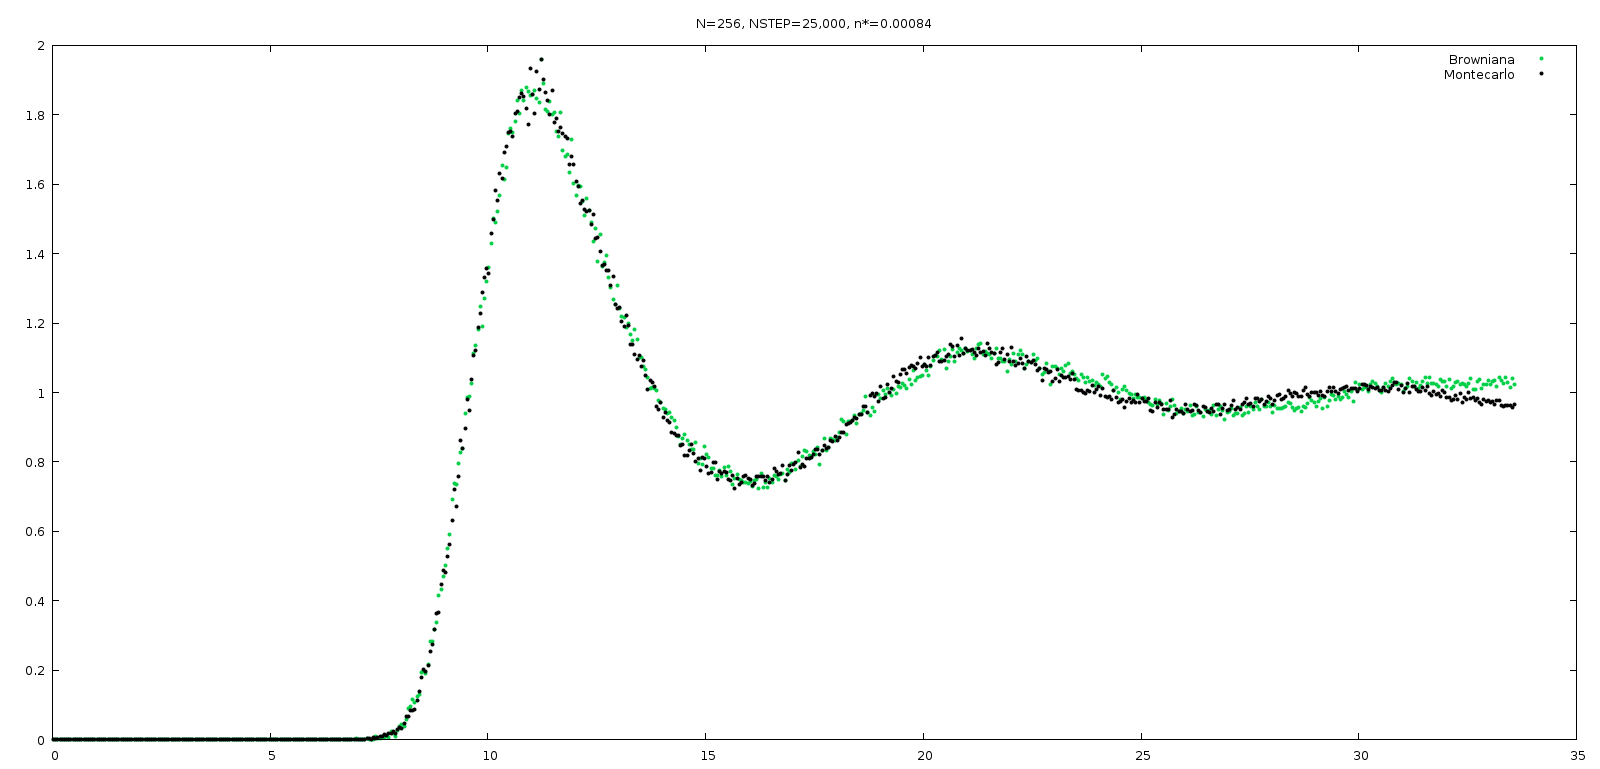
\includegraphics[width=0.75\linewidth]{gdr.png}
	\caption{Función G(r) de la exploración con dinámica molecular.}
\end{figure}


\begin{thebibliography}{widestlabel}
\bibitem{1}  Yeomans, Laura\emph{Guía del curso sobre simulación de dinámica browniana y algoritmo de Verlet (1982)}, Desarrollo experimental, semestre 2018-1.
\end{thebibliography}


\end{document}